% Copyright (C) 2012 Thomas L. Kula
% All Rights Reserved
%
% See the file LICENSE for license terms.
\documentclass[12pt]{article}
\usepackage{graphicx}
\usepackage{rotating}
\usepackage{fix-cm}
\usepackage{multirow}
\setlength{\paperwidth}{5.5in}
\setlength{\paperheight}{8.5in}
\setlength{\textheight}{7.45in}
\setlength{\topmargin}{-1.0in}
\setlength{\oddsidemargin}{-0.5in}
\setlength{\evensidemargin}{-0.5in}
\setlength{\textwidth}{4.0in}
\setlength{\parindent}{0in}
\setlength{\parskip}{3mm}
\usepackage[print]{booklet} \nofiles
\source{\magstep0}{5.5in}{8.5in}
\target{\magstep0}{11in}{8.5in}
\setpdftargetpages
\pagestyle{empty}
\begin{document}


\begin{center}
{\fontsize{36}{48}\selectfont \textsc{Haiku a Day }}
\end{center}

\vspace*{3.5cm}

{\fontsize{20}{40}\selectfont 

A quiet bustle

Fills the city this evening

A honk chastises

}

\vspace*{5.0cm}
\begin{center}
{\large{Issue 81: March 2012}} \\[5mm]
{\fontsize{8}{8}\selectfont  \textsc{ St. Joshua Norton Press }} \\[1mm]
{\fontsize{6}{6}\selectfont Mathom House by the Cloisters \textbar The People's Republic of Ames }
\end{center}


\newpage

It's springtime in Inwood, and this month Random Photo returns.

--- Thomas

http://kula.tproa.net/had/ \\
kula@tproa.net

Download this and previous HADs at the website, so you can
print out your own (DIY, yeah!) or if you want me to send
you one, send me your address, and maybe a stamp if you
are feeling nice. Or send me something you've made ---
trades always appreciated, postcards are nice too.

\vfill

1 March 2012

Piles of data \\
Waiting to be analyzed \\
Filling me with joy

2 March 2012

Groove becomes trenches \\
Solving a problem a fight \\
Mind racing, then win

3 March 2012

Dreary the gray breaks \\
As blue, sliding from the sky \\
Lights the ground below

\newpage

4 March 2012

One less box around \\
A pale victory compared \\
To all the ones left

5 March 2012

Lightbulbs blowing out \\
Not used to that happening; \\
So rare now these days

6 March 2012

Flash crashing this site \\
Lots of sad puzzle pieces \\
I kick Chrome; go on

7 March 2012

Through the Fog of Code \\
On the other side, sitting \\
Pure lucidity

8 March 2012

Bright knot in my back \\
You have no reason to be \\
Go away now, please

9 March 2012

Files flashing by \\
As data from here to there \\
Shuffles through the net

10 March 2012

Strong taco cravings \\
Can only lead to one thing \\
Strong taco eating

\newpage

11 March 2012

Fingernails creep me \\
Dead things growing from the ends--- \\
Shit! There's toenails too?

12 March 2012
 
Subway, rocking, lulls \\
Me with the promise of sleep \\
Must not fall for it

13 March 2012

Ignoble Pigeons \\
Divebombing, miss the sidewalk \\
Fly away, unmissed

14 March 2012

Do you hear the song? \\
Scored a million players strong \\
City Symphony

15 March 2012

The crave for a slice \\
Is a strong longing today \\
No pizza this week

16 March 2012

Falafel Friday \\
So sublime in its beauty \\
In purpose, noble

17 March 2012

Layers and weaving \\
A warm dark cave in softness \\
Makes a place to sleep

\newpage

18 March 2012

Run out of coffee \\
Time to get the day going \\
Many things to do

19 March 2012

Quiet thoughts nagging \\
In the back of the head break \\
Through and make antsy

20 March 2012

Beware the sidewalks \\
Angry with all the stepping \\
They try to trip you

21 March 2012

Streetside sentinals \\
Watching you, counting seconds \\
Their wrath brings tickets

22 March 2012

The thunk of relays \\
Keeping me safe each morning \\
Holding back traffic

23 March 2012

Metal oracles \\
Divine wisdom in the air \\
Providing guidance

24 March 2012

Giant bee buzzing \\
In my living room, confused \\
Windows confound it


\newpage

25 March 2012

Somedays, Sundays fill \\
With rapt productivity \\
That is not today

26 March 2012

Zigzag lines growing \\
Foreshadowing a migraine \\
Only a shadow

27 March 2012

I'm often surprised \\
At how quiet it can be \\
Inside the city

28 March 2012

Walking through the park \\
On a cool, early Spring day \\
The world is all right

29 March 2012

I hear a faint beep \\
And a forlorn buzzing sound \\
Coming down the street

30 March 2012

Not a welcome sound, \\
The motorcycle assholes \\
Tearing through the night

31 March 2012

Stuck here at the end \\
Thirty-one days passing by \\
Tomorrow: April

\newpage

\begin{center}
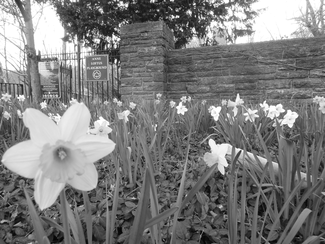
\includegraphics[width=325pt]{inwood.png}

Dafodills at Anne Loftus Playground \\
Inwood, Manhattan \\
{\tt kula.tproa.net/photos/2012/20120319-inwood-spring/ }
\end{center}

\newpage

\thispagestyle{empty}
\vspace*{12cm}
\begin{sideways}
\Large{St. Joshua Norton Press}
\end{sideways}
\begin{sideways}
\Large{PO Box 250138}
\end{sideways}
\begin{sideways}
\Large{New York NY 10025}
\end{sideways}


\end{document}


